\begin{titlepage} % Suppresses displaying the page number on the title page and the subsequent page counts as page 1
	\newcommand{\HRule}{\rule{\linewidth}{0.5mm}} % Defines a new command for horizontal lines, change thickness here
	
	\center % Centre everything on the page
	
	%------------------------------------------------
	%	Headings
	%------------------------------------------------
	
	\textsc{\LARGE IDPA 2018-2019}\\[1.5cm] % Main heading such as the name of your university/college
	
	\textsc{\Large Wie wir uns gewehrt hätten}\\[0.5cm] % Major heading such as course name
	
	%------------------------------------------------
	%	Title
	%------------------------------------------------
	
	\HRule\\[0.4cm]
	
	{\huge\bfseries Eine wehrhafte Schweiz}\\[0.4cm] % Title of your document
	
	\HRule\\[1.5cm]
	
	%------------------------------------------------
	%	Author(s)
	%------------------------------------------------
	
	%\begin{minipage}{0.4\textwidth}
	%	\begin{flushleft}
	%		\large
	%		\textit{Autoren}\\
     %       Stefanie \textsc{Jäger} % Your name
      %      
        %	Seya \textsc{Schmassmann} % Your name
		%	
		%\end{flushleft}
	%\end{minipage}
	%~
	%\begin{minipage}{0.4\textwidth}
	%	\begin{flushright}
	%		\large
	%		\textit{}\\
     %       Dario \textsc{Wigger} % Your name
      %      
		%	Joel \textsc{Wälti} % Your name
		%\end{flushright}
	%\end{minipage}
	
	% If you don't want a supervisor, uncomment the two lines below and comment the code above
	{\large\textit{Autoren}}\\
	Stefanie Jäger, % Your name
	Seya Schmassmann, % Your name
	Dario Wigger und % Your name
	Joel Wälti % Your name
	%------------------------------------------------
	%	Date
	%------------------------------------------------
	
	\vfill\vfill\vfill % Position the date 3/4 down the remaining page
	
	{\large IDPA 2019, Berufsfachschule BBB Berufsmaturität} % Date, change the \today to a set date if you want to be precise
	
	%------------------------------------------------
	%	Logo
	%------------------------------------------------
	
	\vfill\vfill
	\begin{figure}[h]
		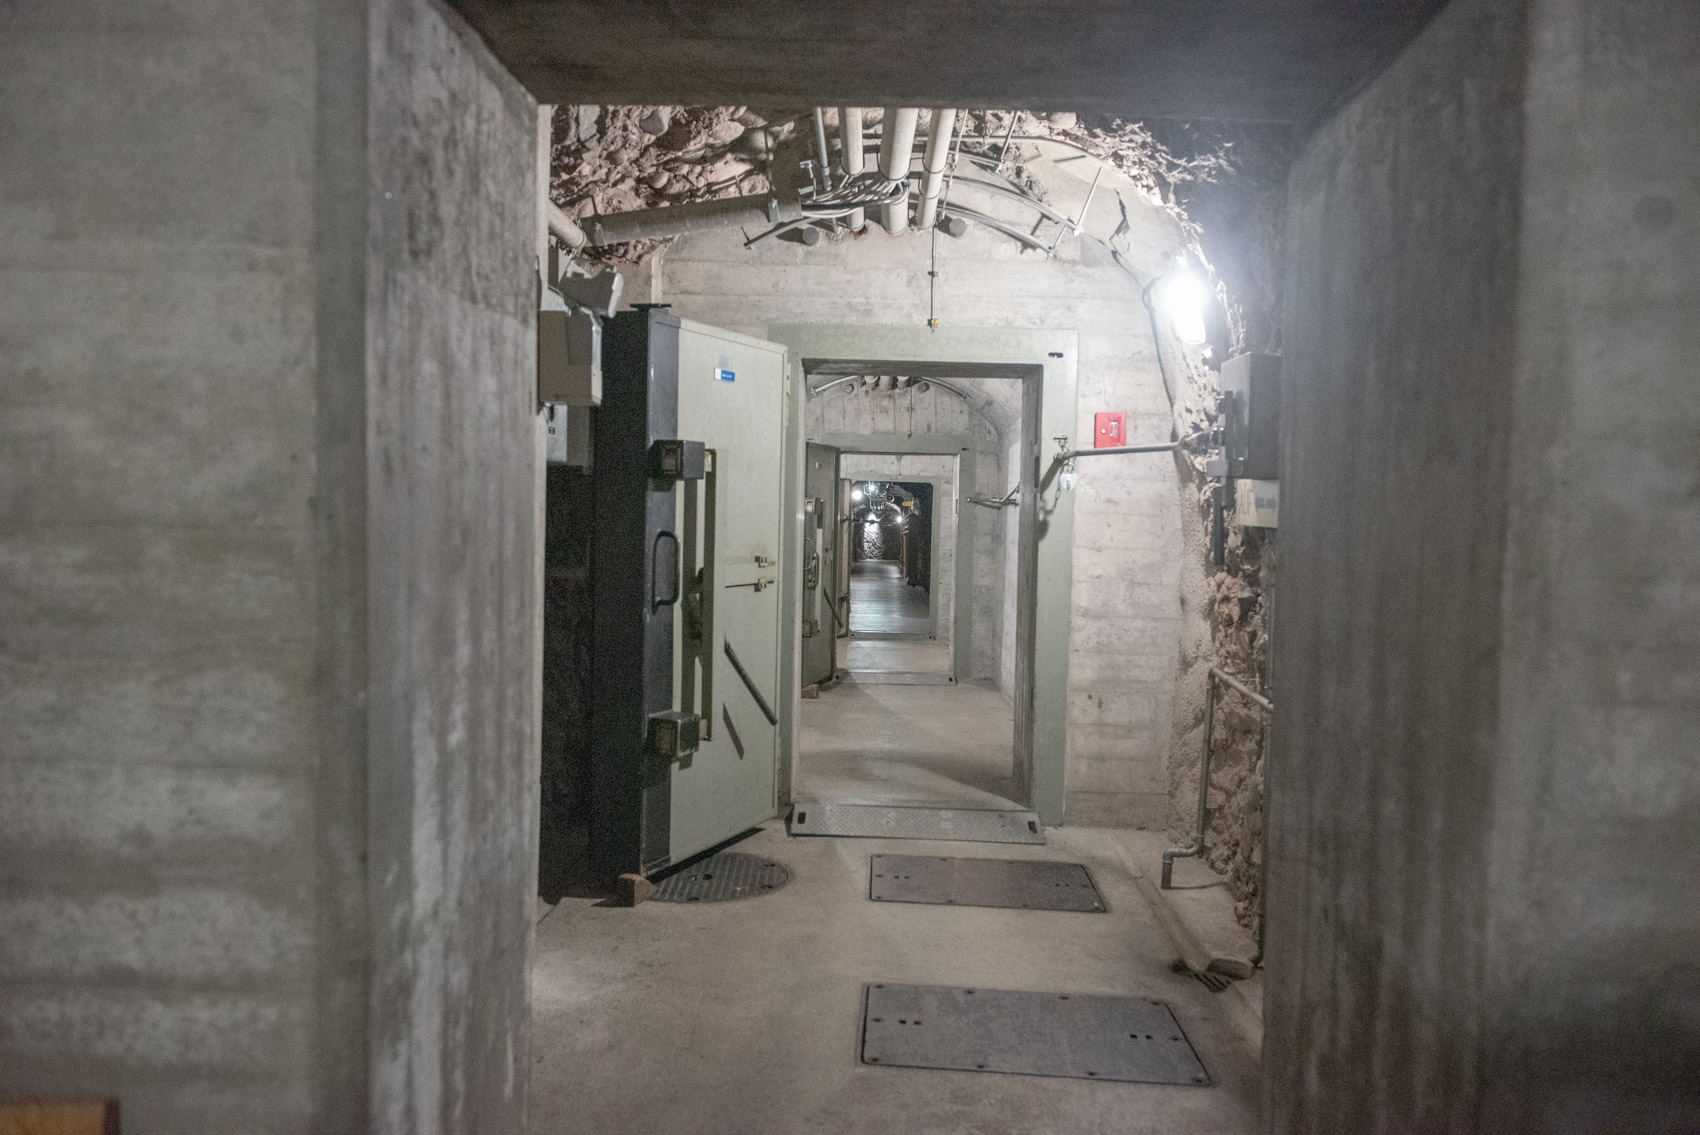
\includegraphics[width=1\textwidth]{images/Fotos_Vitznau_085.jpg} % Include a department/university logo - this will require the graphicx package
		\caption[{Seya Schmassmann (2019). Gang der Festung Vitznau (27. April 2019). [Stand 24.08.2019] }] {Gang der Festung Vitznau}
	\end{figure}
		
	%----------------------------------------------------------------------------------------
	
	\vfill % Push the date up 1/4 of the remaining page
	
\end{titlepage}